\capitulo{5}{Resultados}

\section{Resumen de resultados.}

\subsection{Resultados plan entrenamiento de Contour}

Tras completar todo el ciclo de actividades, las cuales consisten en un programa de entrenamiento con una duración de 10 días, los profesionales de Contour analizaron los datos y han generado un informe individual. Los datos permanecen anónimos y cada persona únicamente verá sus propios resultados individuales y además, datos generales de otros miembros de la comunidad de manera anónima. Estos resultados se pueden dividir en 3 tipos de análisis: de la eficiencia cognitiva como en la imagen \ref{fig: ContourCognitiveEfficiency}, del tiempo transcurrido en un estado de concentración óptima como la imagen \ref{fig: ContourTimeSpent} y del estado de ánimo del usuario antes y después de realizar las actividades como en la imagen \ref{fig: ContourDailyStatus}.

\newpage
\begin{figure}[h]
    \centering
    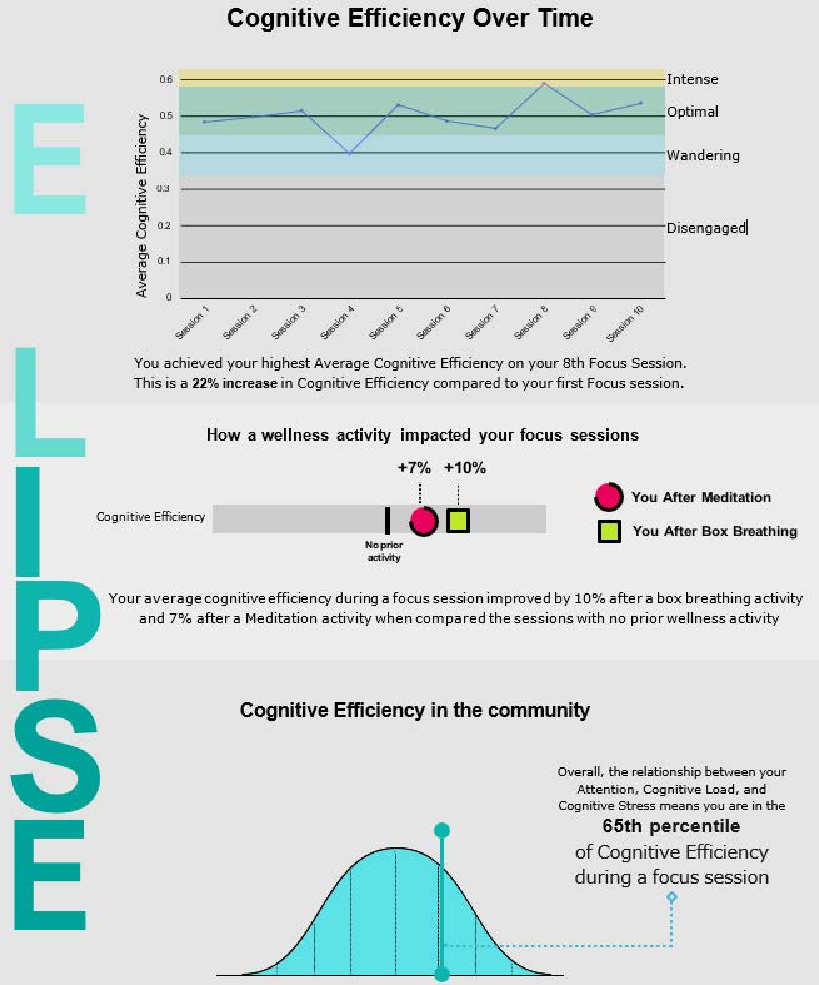
\includegraphics[width=0.9\textwidth]{img/ContourCognitiveEfficiency.pdf}
    \caption{Resultados del análisis de la eficiencia cognitiva durante el programa de entrenamiento de 10 días.}
    \label{fig: ContourCognitiveEfficiency}
    \end{figure}

\begin{figure}[H]
    \centering
    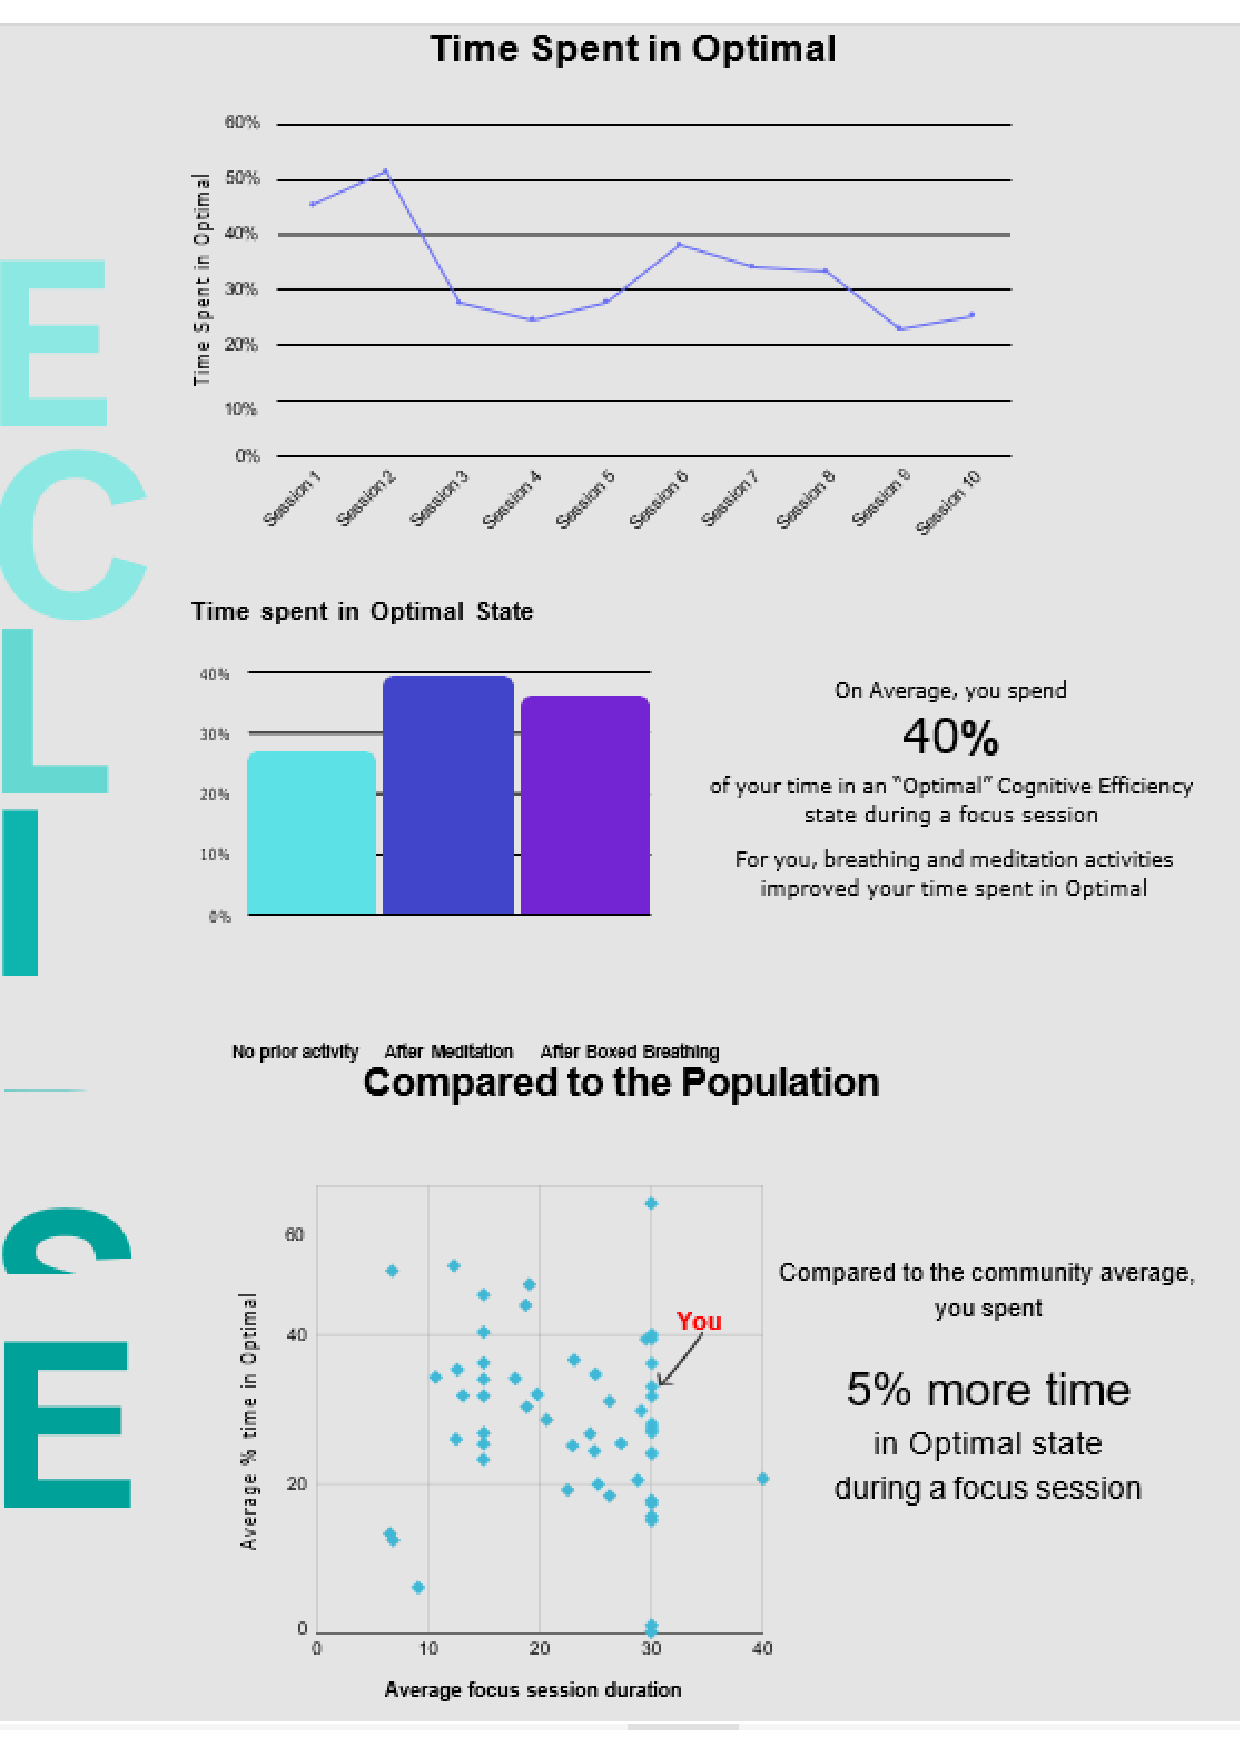
\includegraphics[width=0.9\textwidth]{img/ContourTimeSpent.pdf}
    \caption{Resultados del análisis del tiempo transcurrido con una concentración óptima durante el programa de entrenamiento de 10 días.}
    \label{fig: ContourTimeSpent}
    \end{figure}

\begin{figure}[H]
    \centering
    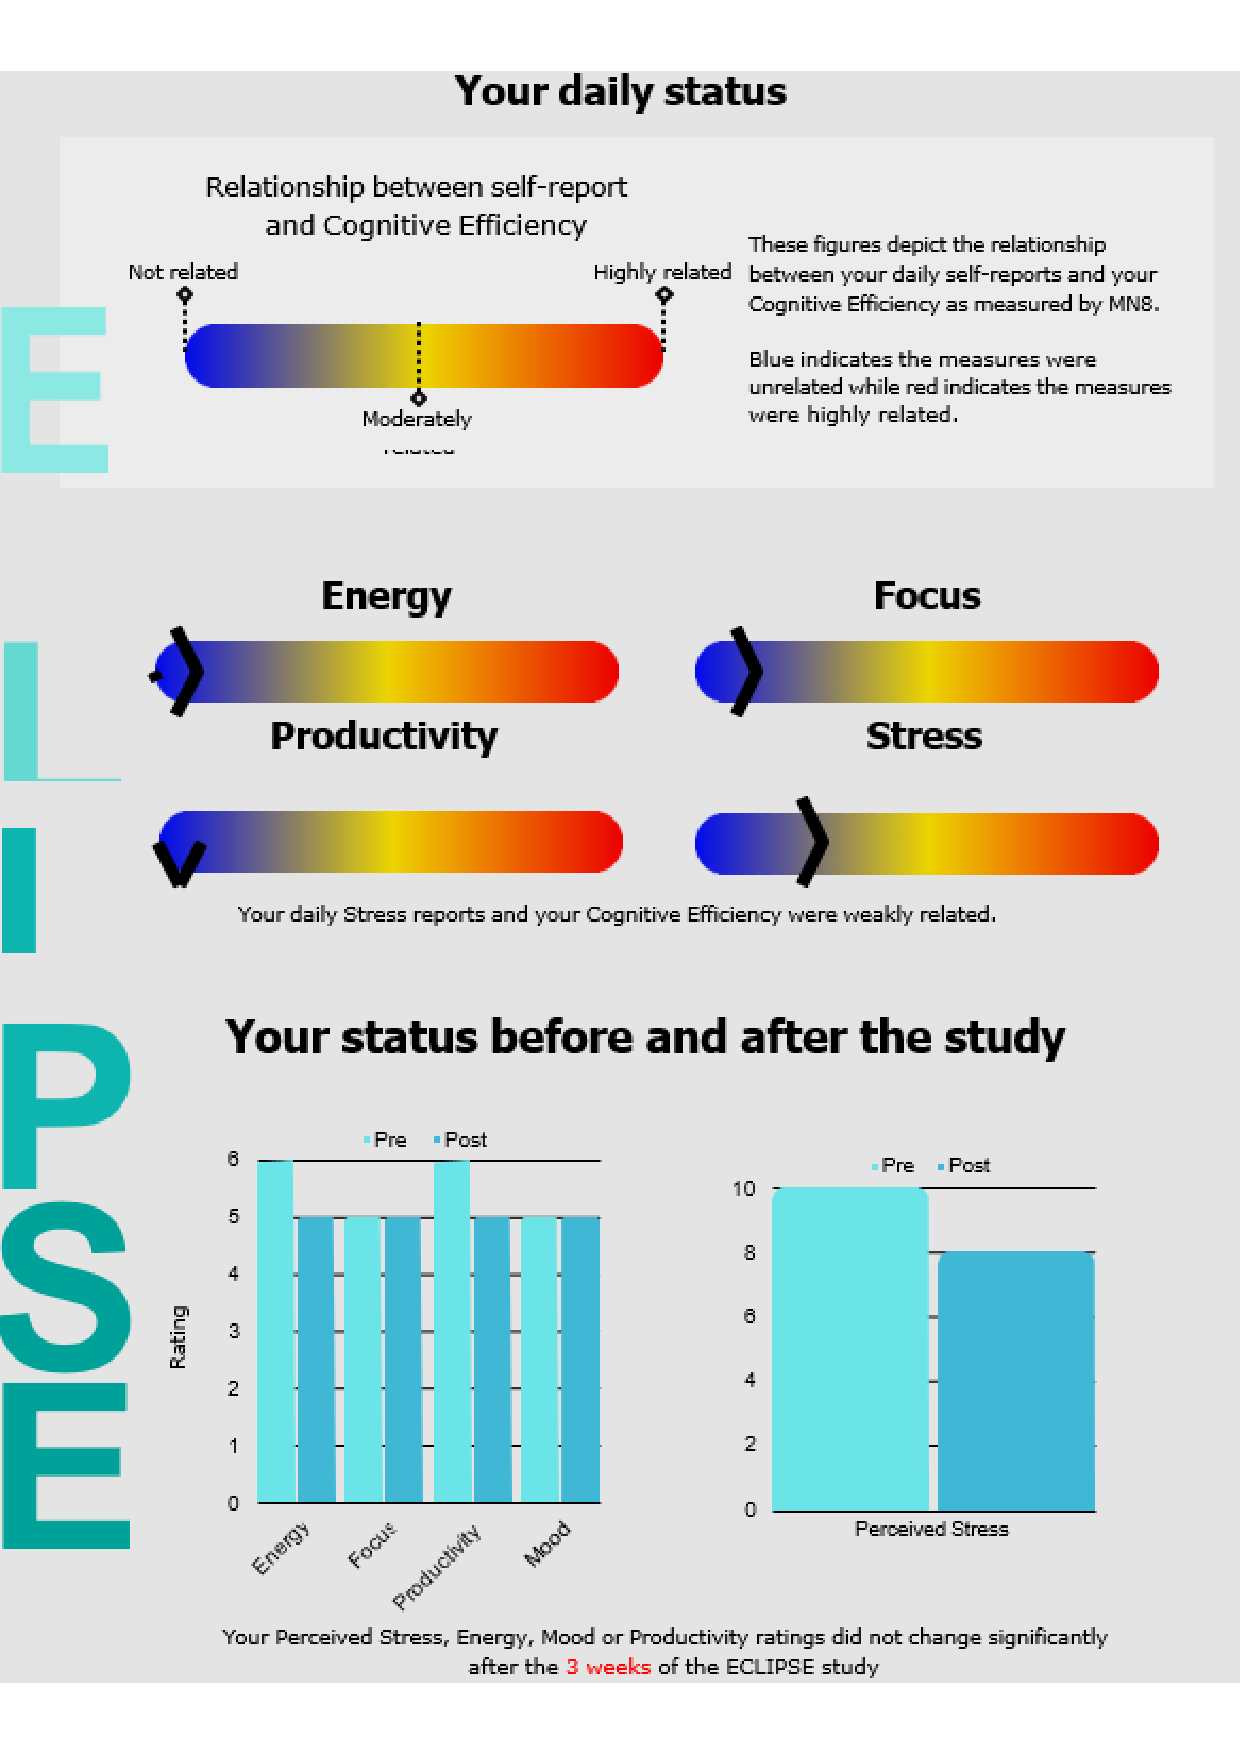
\includegraphics[width=0.9\textwidth]{img/ContourDailyStatus.pdf}
    \caption{Resultados del análisis del estado de ánimo del usuario durante el programa de entrenamiento de 10 días.}
    \label{fig: ContourDailyStatus}
    \end{figure}

\subsection{Resultados sesión meditación de PsychoPy}

Después de realizar el experimento diseñado en PsychoPy, se debería de obtener una grabación almacenada en EmotivPRO, la cual deberá ser exportada a un archivo para el tratamiento de los datos. El formato más adecuado para trabajar sobre ellos es CSV, ya que permite la visualización de todos los valores en forma de filas y columnas.

En el caso del experimento creado, no se pueden obtener resultados de grabaciones ya que el dispositivo MN8 no llega a conectarse con la aplicación de PsychoPy. Esto no se debe a un problema de programación, si no que se debe a algún problema relacionado con el \textit{software} desconocido y sin documentación sobre ello. Por lo tanto, en la imagen \ref{fig: ResultadosExperimentoYoutube} obtenida de \cite{VideoExperimentoMN8PsychoPy}\footnote{Vídeo de Youtube con el tutorial de realización de un experimento en PsychoPy empleando el MN8 \cite{VideoExperimentoMN8PsychoPy}.}, en el que se muestran los resultados de un experimento de PsychoPy, también emplea un dispositivo MN8 y así se puede observar como se visualizan los resultados de la grabación en un archivo CSV.

\begin{figure}[H]
    \centering
    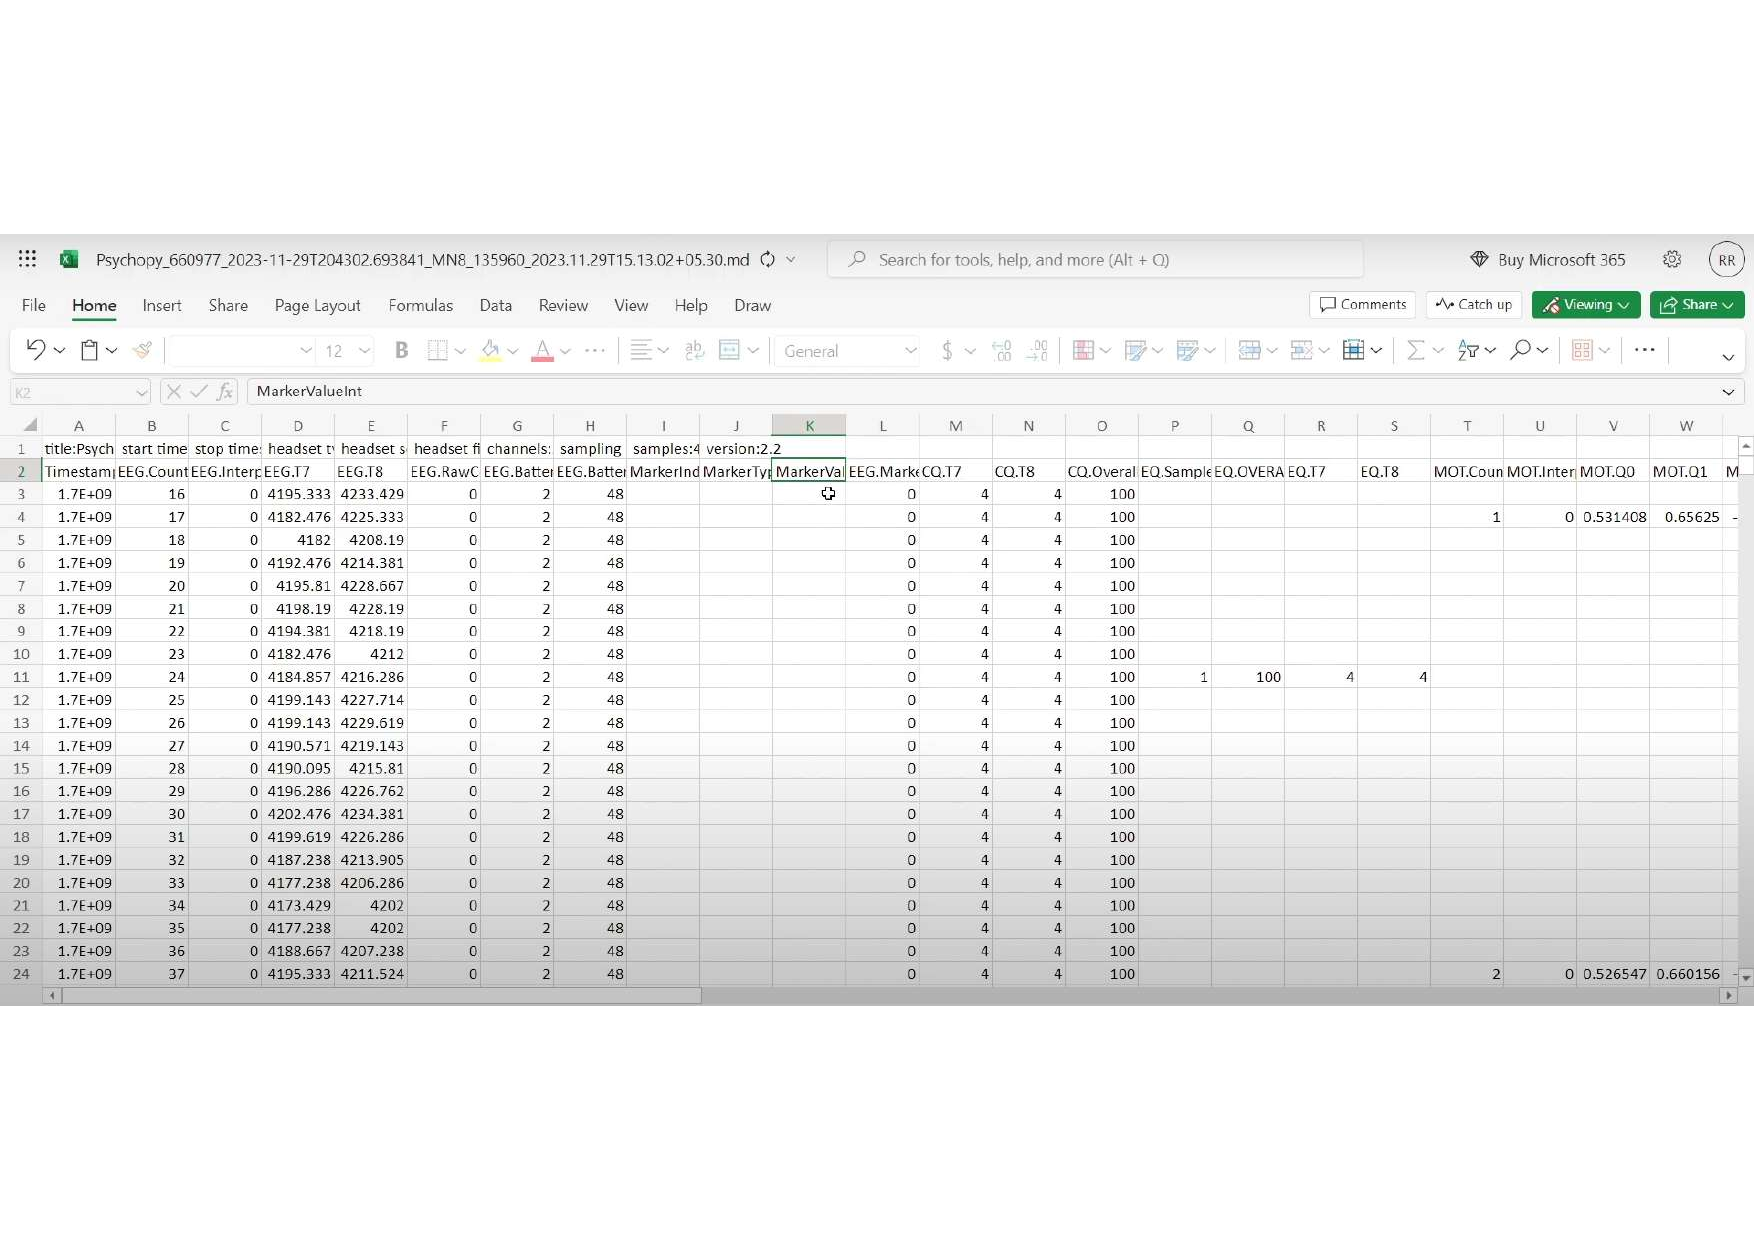
\includegraphics[width=1.2\textwidth]{img/ResultadosExperimentoYoutube.pdf}
    \caption{Resultados de un experimento de PsychoPy empleando Emotiv MN8 obtenido de \cite{VideoExperimentoMN8PsychoPy}.}
    \label{fig: ResultadosExperimentoYoutube}
    \end{figure}

\section{Discusión.}

Se ha estado investigando sobre el error producido en el experimento realizado y consiste en una pantalla en negra cuando se ejecuta el mismo. Esta pantalla negra se genera porque la aplicación está intentando conectarse con el MN8 pero no lo consigue, por lo que se queda constantemente en la pantalla hasta que se cierre manualmente el experimento. Por más que se haya investigado en las páginas y documentaciones de Emotiv y de PsychoPy, no hay nada relacionado con este error, por lo que se ha llegado a la conclusión de que es un problema de conexión entre los componentes, la cual no tiene ninguna relación con la manera en la que se ha implementado el código en bloques.

En el caso del correcto funcionamiento de este experimento, se obtendría una grabación similar a la de la imagen \ref{fig: ResultadosExperimentoYoutube}, en la que aparecen los valores a lo largo del experimento de los 2 canales registrados, así como el porcentaje de batería, el porcentaje de la calidad de la señal y otros valores de distintos parámetros.

Los diferentes dispositivos de Emotiv permiten medir la actividad cerebral y su posterior análisis para detectar sensaciones, acciones o incluso enfermedades. Por ejemplo, en la investigación \cite{ArticuloDiscusion1}\footnote{Artículo de la investigación sobre el Emotiv EPOC \cite{ArticuloDiscusion1}.} se utiliza la diadema Emotiv EPOC de 14 canales para detectar la emoción del miedo. Para ello sólo fueron necesarios 4 de los 14 canales, situados en la parte frontal. Para la obtención de resultados se normalizaron los valores que se obtienen y se representan en una gráfica con etiquetas para cada emoción, pudiendo observar los resultados antes del estímulo de miedo en la imagen \ref{fig: EEGReposoDiscusion1} y los resultados después del estímulo en la figura \ref{fig: EEGMiedoDiscusion1}.

\begin{figure}[h]
    \centering
    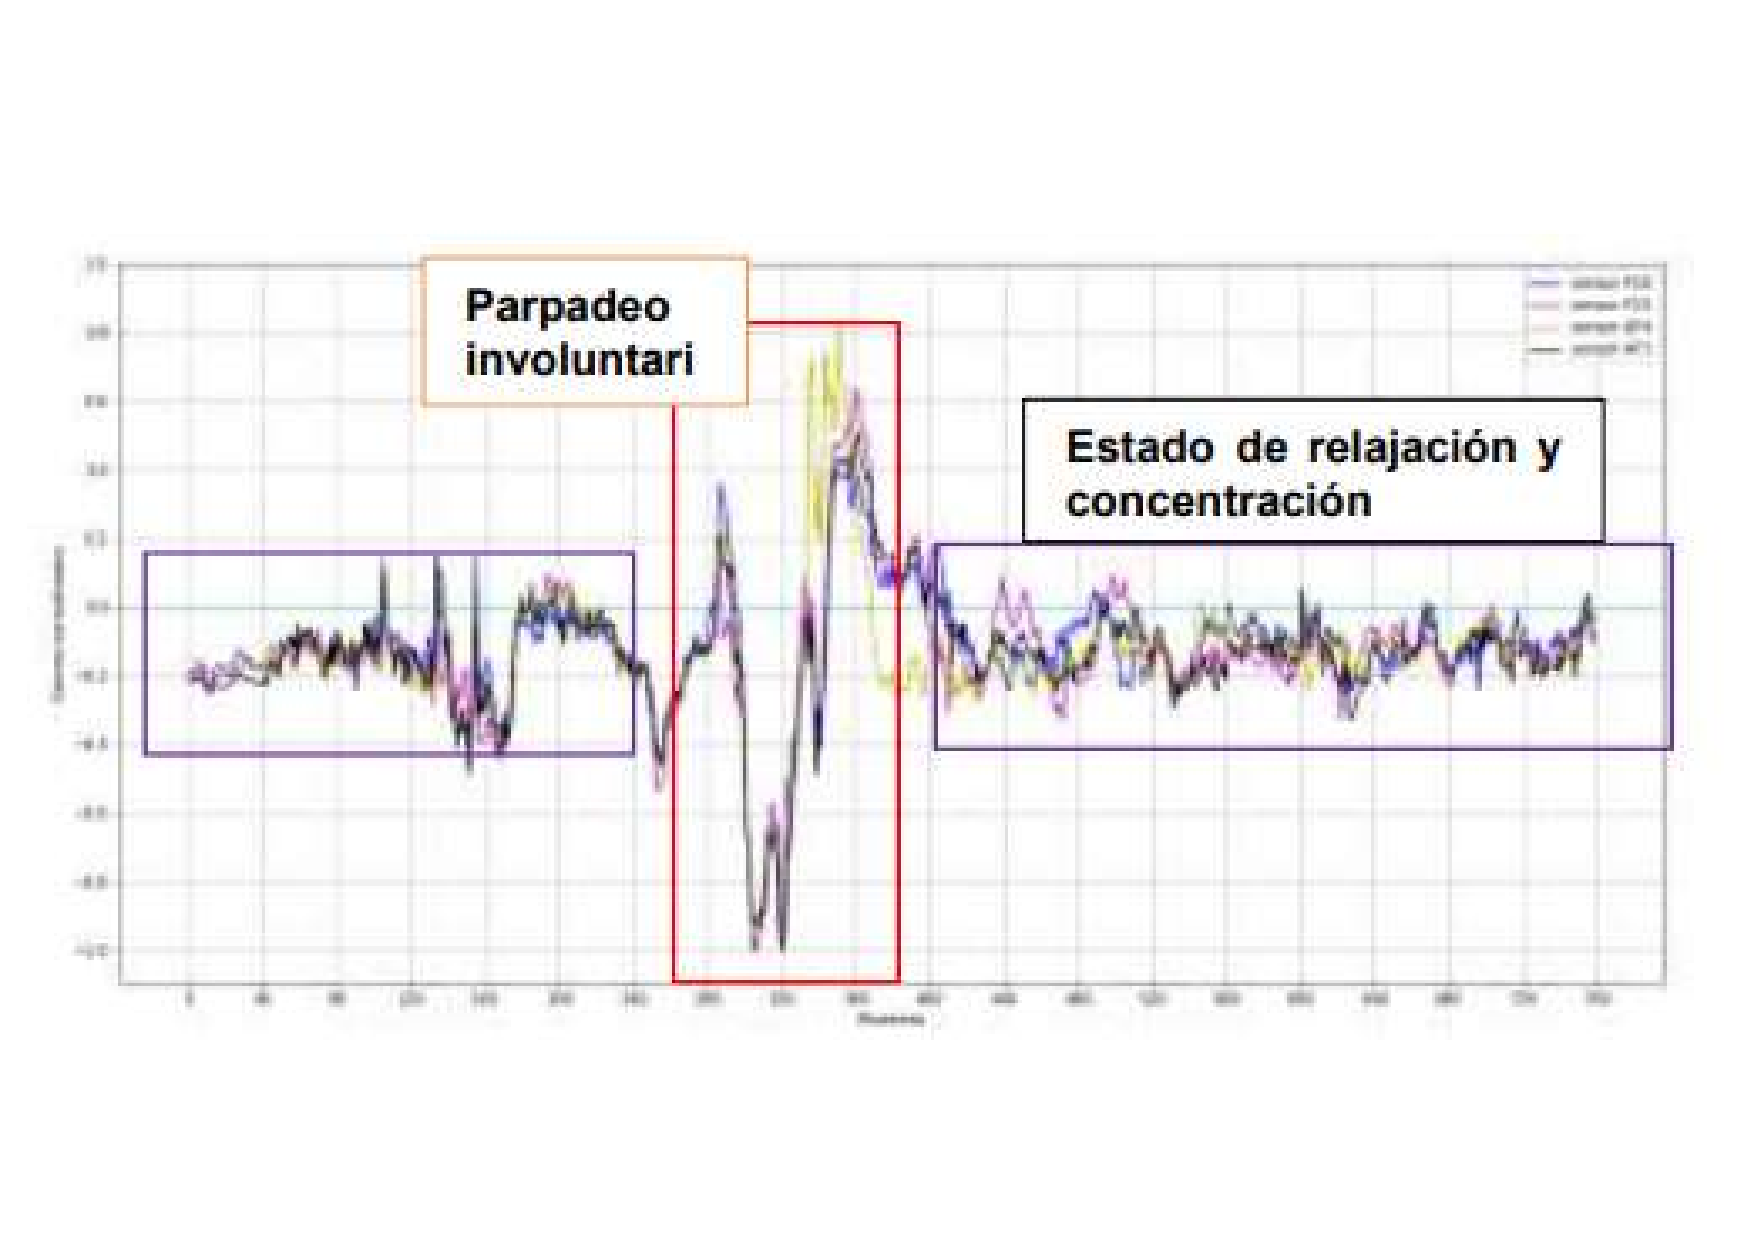
\includegraphics[width=0.9\textwidth]{img/EEGReposoDiscusion1.pdf}
    \caption{Resultados de un experimento empleando el Emotiv EPOC antes de estímulo de miedo.}
    \label{fig: EEGReposoDiscusion1}
    \end{figure}

\begin{figure}[h]
    \centering
    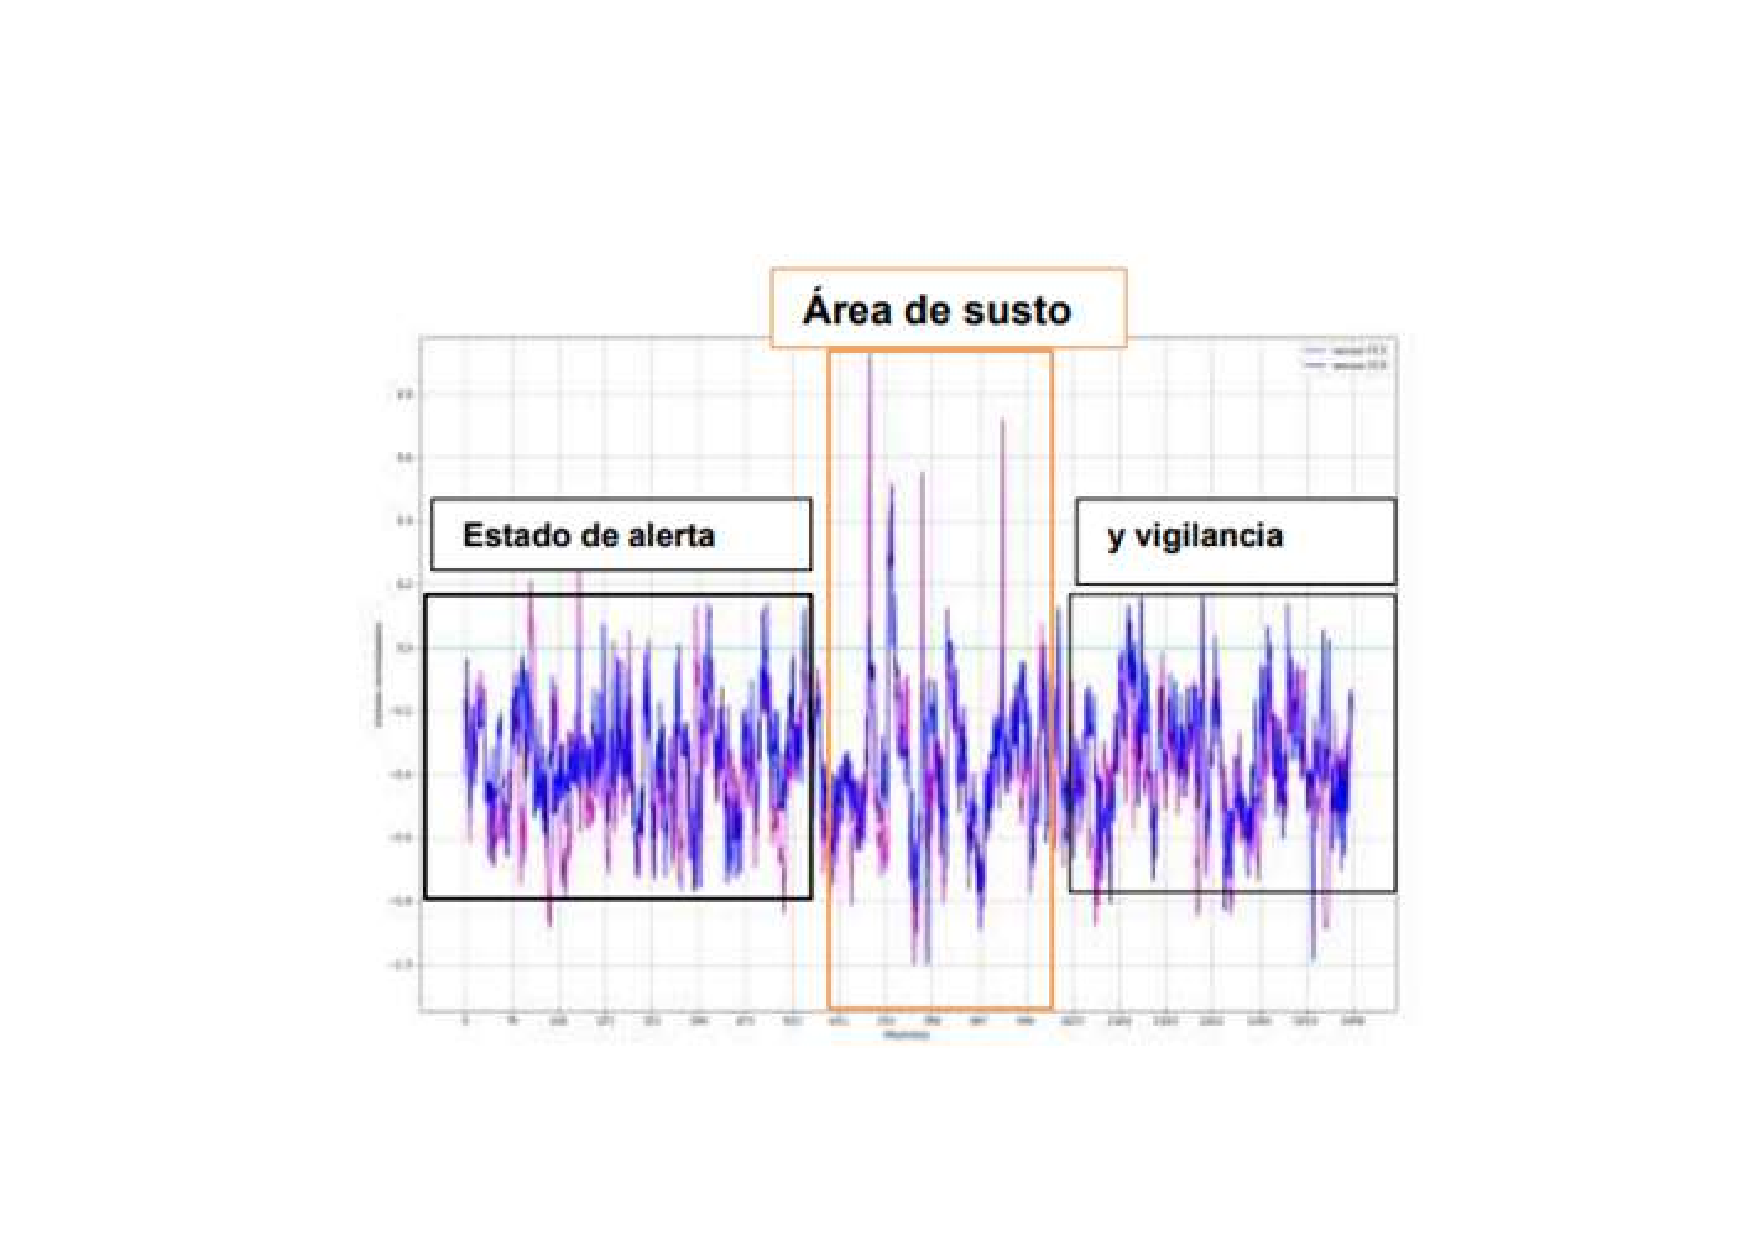
\includegraphics[width=0.9\textwidth]{img/EEGMiedoDiscusion1.pdf}
    \caption{Resultados de un experimento empleando el Emotiv EPOC después de estímulo de miedo.}
    \label{fig: EEGMiedoDiscusion1}
    \end{figure}

Otro proyecto similar es el del artículo \cite{ArticuloDiscusion2}\footnote{Segundo artículo de la investigación sobre el Emotiv EPOC \cite{ArticuloDiscusion1}.}, que mide la actividad cerebral de un sujeto mientras juega a videojuegos y relaciona los elementos del juego con emociones. Para ello se utiliza de nuevo el dispositivo Emotiv EPOC y mediante una serie de transformaciones en los valores para interpretar las emociones llega a la tabla de la imagen \ref{fig: TablaDiscusion2}.

\begin{figure}[h]
    \centering
    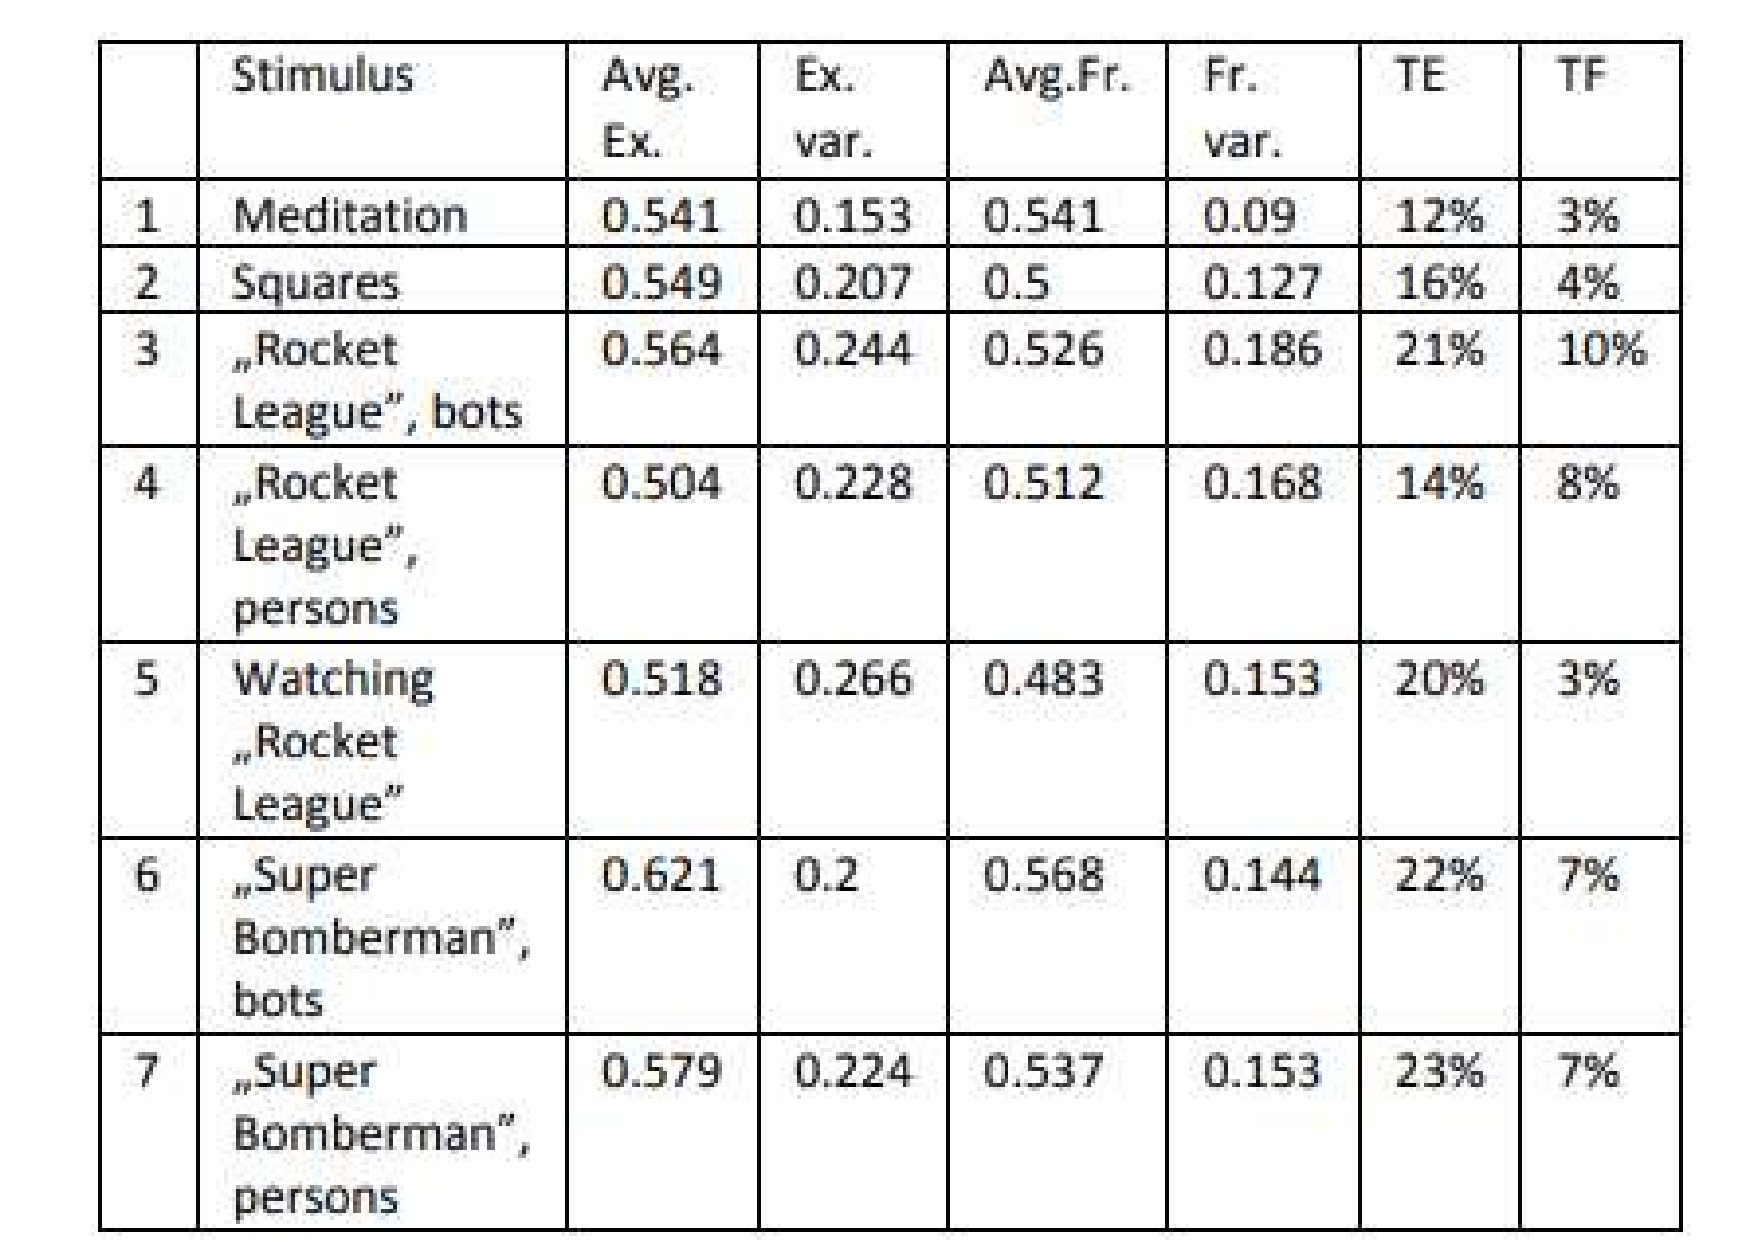
\includegraphics[width=0.7\textwidth]{img/TablaDiscusion2.pdf}
    \caption{Tabla con los valores obtenidos en cada videojuego.}
    \label{fig: TablaDiscusion2}
    \end{figure}

Para mostrar los resultados, como en el anterior, muestra la gráfica de la figura \ref{fig: EEGDiscusion2} con etiquetas que definen el sentimiento predominante en momento de la partida.

\begin{figure}[h]
    \centering
    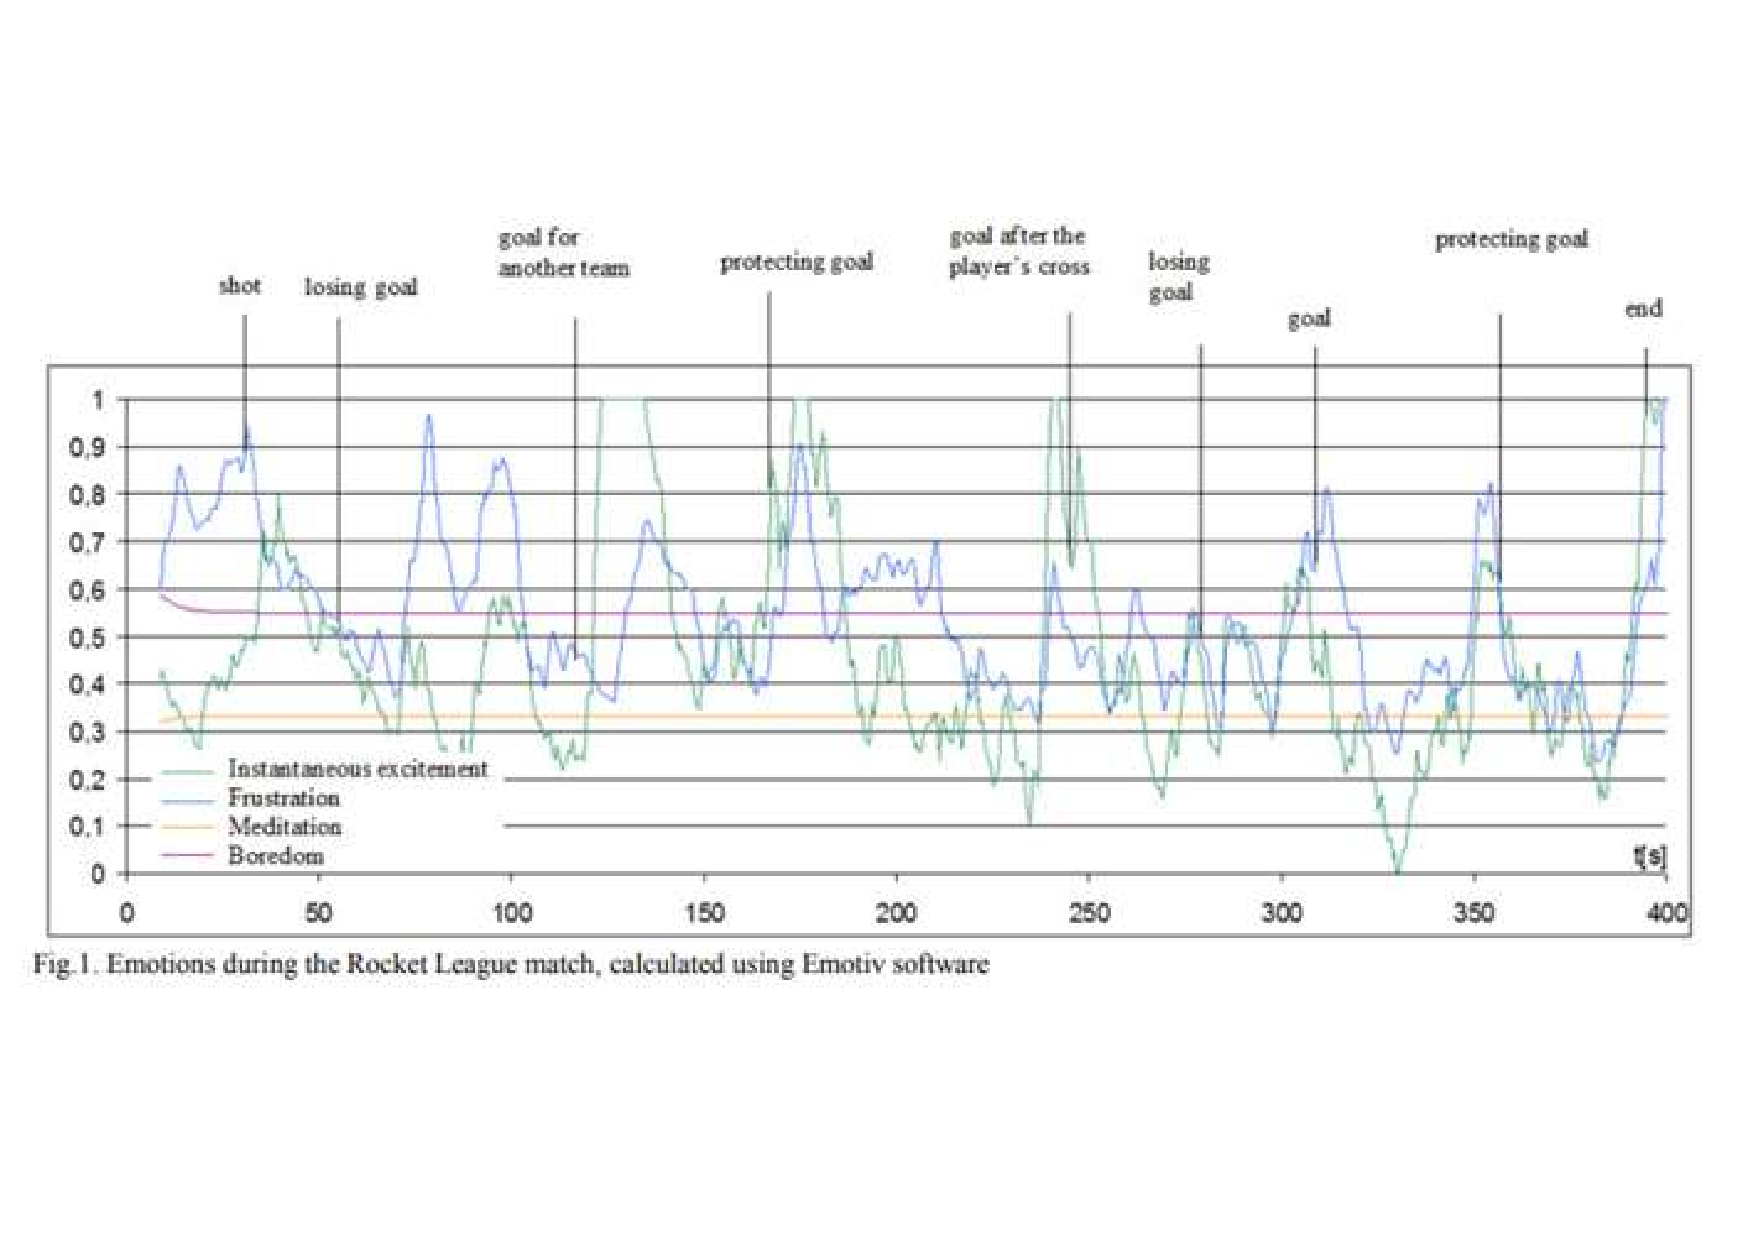
\includegraphics[width=0.7\textwidth]{img/EEGDiscusion2.pdf}
    \caption{EEG del usuario a lo largo de la partida.}
    \label{fig: EEGDiscusion2}
    \end{figure}
